% Chapter 

\chapter*{Conclusion} % Main chapter title

\label{Conclusion} % For referencing the chapter elsewhere, use \ref{Chapter1} 

% \lhead{Chapter 1. \emph{Introduction}} % This is for the header on each page - perhaps a shortened title

\graphicspath{{./Pictures/}}

%----------------------------------------------------------------------------------------
\newcommand*\circled[1]{\tikz[baseline=(char.base)]{\node[shape=circle,draw,black,inner sep=0.3pt] (char) {#1};}}

The release of non-enveloped viruses has been for a long time considered a passive process associated with cellular lysis. Recently, there is growing evidence suggesting an active mechanism for the egress of non-enveloped progeny virions, thus challenging the current basic principle in virology. However, the mechanism involved remains elusive. The current knowledge concerning nuclear maturation, export, and egress of non-enveloped viruses is limited. The main aim of this thesis was to confirm the existence of an active mechanism of egress and to identify the late nuclear maturation steps of minute virus of mice (MVM) leading to nuclear export of the virion progeny. 
    
\par
\medskip
Anion-exchange chromatography (AEX) was performed to separate intracellular virus populations displaying different protein surface configurations. Apart from empty capsids (EC), two well defined DNA-containing populations were separated based on their net surface charges. The full capsid (FC) populations, referred to as FC-P\textsubscript{1} and FC-P\textsubscript{2}, differed in the conformation of their N-termini of the viral capsid protein VP2 (N-VP2), as well as in their surface phosphorylation status. Nuclear export and active egress prior to cytolysis was observed only for the late FC-P\textsubscript{2} population. The segregation of the two FC populations confirms an active mechanism of egress. While N-VP2 was not involved in the active nuclear export of MVM, the surface phosphorylations were strictly associated with nuclear export. During their life cycle, karyophilic viruses need to master a bidirectional nuclear transport, wherein early in infection, the virus is imported into the nucleus where it hijacks the replication machinery of the host cell. Following assembly and DNA-packaging, progeny virions are exported from the nucleus. In order to achieve this paradoxical situation, the virus needs to rearrange its capsid surface to acquire nuclear import or export potential. 


\par
\medskip
Our findings revealed spatially and temporally controlled modifications of capsid surface phosphorylations (see Figure~\ref{Scheme}, p.~\pageref{Scheme}) as a pivotal mechanism mediating nuclear import and export of a karyophilic virus. 






\begin{figure}[H]
\centering
  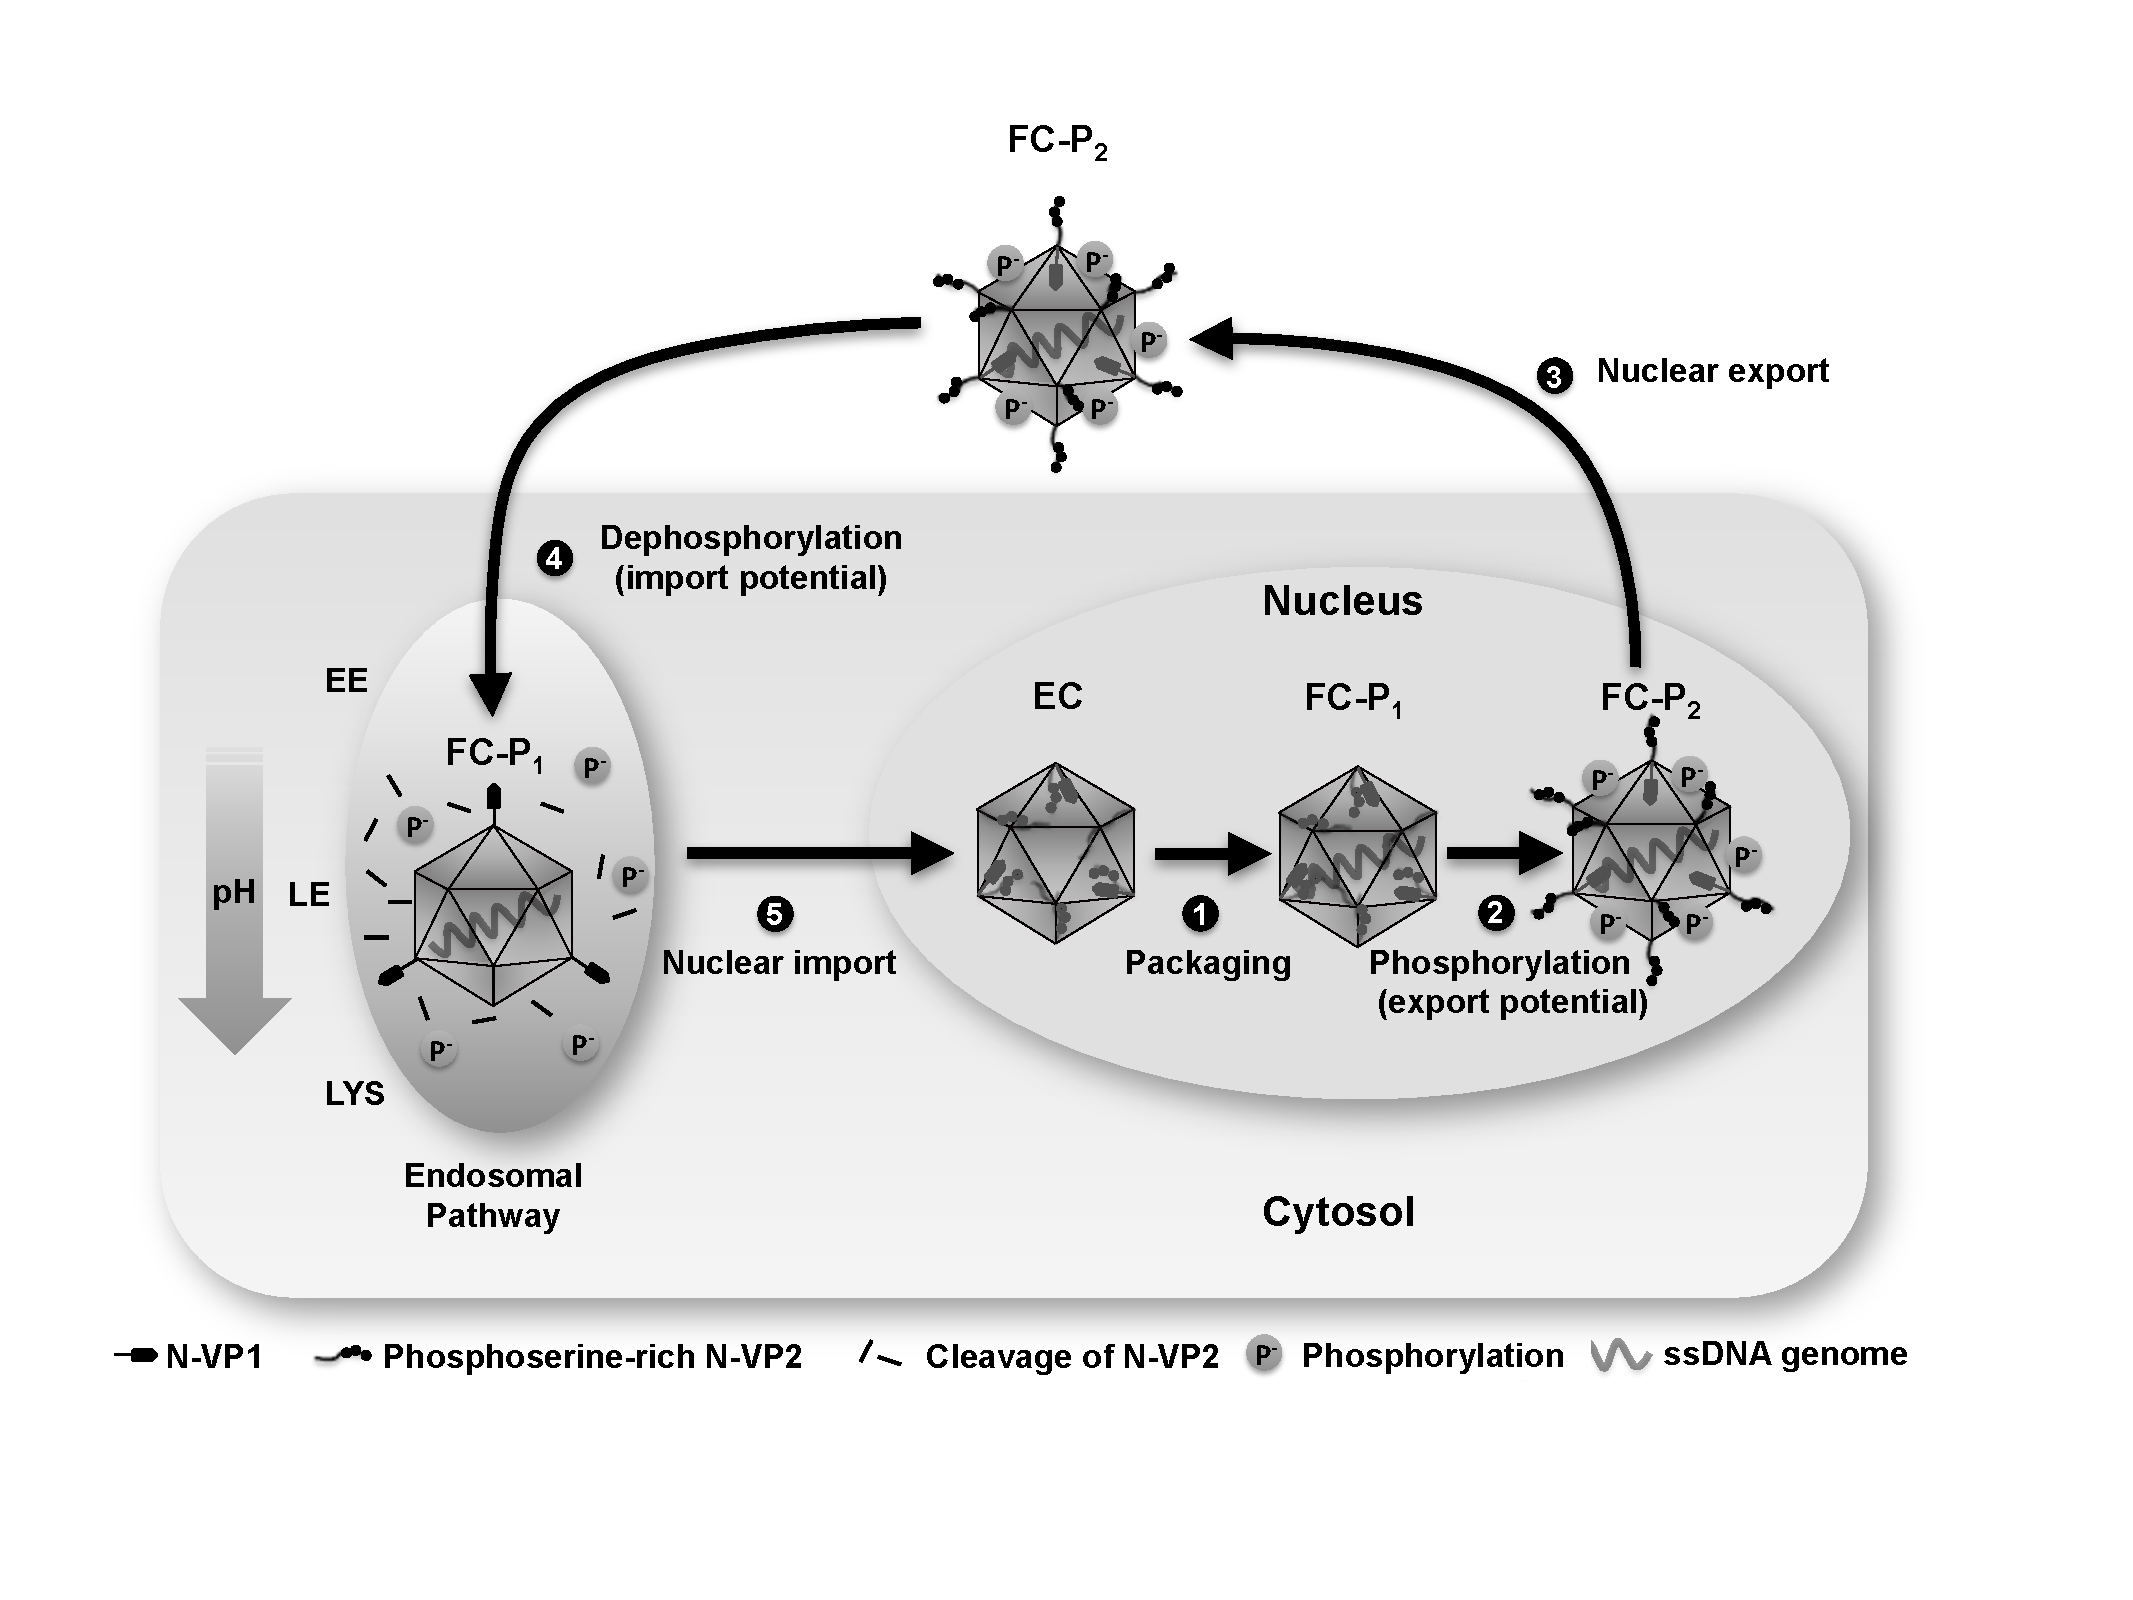
\includegraphics[trim = 0mm 0mm 5mm 0mm, width=0.9\textwidth]{Conclusion}\\[0.2cm]
  \caption[Model of Nuclear Import and Export of MVM]
   {Model of nuckear import and export of MVM. Surface phosphorylations play a pivotal role in determining the nuclear export of MVM. \textbf{\circled{1}}~During entry, the surface phosphorylations of export competent FC-P\textsubscript{2} virions are removed by acidic phosphatases, adopting the FC-P\textsubscript{1} phsophorylation pattern. \textbf{\circled{2}}~Infectious incoming virions escape the endosomal pathway and are imported into the nucleus. \textbf{\circled{3}}~Following self-assembly of the structural proteins, the empty capsids (EC) are filled with a ssDNA genome, leading to the generation of FC-P\textsubscript{1} virions. \textbf{\circled{4}}~FC-P\textsubscript{1} particles are phosphorylated by a nuclear kinase, resulting in the accumulation of FC-P\textsubscript{2} virion progeny. \textbf{\circled{5}}~FC-P\textsubscript{2} virions are exported from the nucleus of infected cells and egress the host cell. The most important capsid elements involved in the viral life cycle are explained below the representation.} 
\label{Scheme}
\end{figure}















% Recent research in our lab focused on dynamics and structural rearrangements on the surface of parvovirus capsids during the first stages of an infection. The studies were conducted on both parvoviruses B19V and MVM. For the latter model virus, three major pH-dependent structural capsid rearrangements were observed \textit{in vivo}. These include the proteolytic digestion of N-VP2, the externalization of N-VP1 through the cylindrical 5-fold channel, and the externalization of viral DNA which remained associated to the capsid (see Section~\ref{Rearrangements}, p.~\pageref{Rearrangements}) \cite{pmid16379002}. To date, neither the triggers causing these endosomal rearrangements nor their purpose have been elucidated in detail. B19V has been shown to undergo conformational changes upon binding to its primary attachment receptor globoside (Gb4Cer), also referred to as erythrocyte P antigen. Binding to the receptor triggers the externalization of VP1u, the highly immunogenic N-terminus of the minor structural capsid protein VP1 \cite{pmid20826697}. VP1u has been shown to be the key determinant for the extraordinarily restricted B19V tropism \cite{pmid24067971}. Most recent results obtained in our lab indicate that B19V undergoes phosphorylation events during cytoplasmic trafficking leading to significant structural rearrangements of the B19V capsid and eventual DNA externalization. While incoming cytoplasmic capsids lost the conformational epitopes targeted by an antibody against assembled capsids, antibodies against phosphorylated serine residues efficiently recognized partially disassembled intermediates. The capsid-tethered genomic DNA of these partially uncoated particles was accessible for \textit{in vitro} extension with specific primers complementary to both ITRs. (Ruprecht, N. \textit{et al.}, manuscript in preparation).  

% As previously mentioned, parvoviruses are highly robust in the extracellular milieu resisting harsh physicochemical conditions (see Section~\ref{Physicoprop}, p.~\pageref{Physicoprop}). However, \textit{in vivo} they need to uncoat their capsid shell in order to ensure an efficient transmission of their genomic DNA into the host’s nucleus. These structural rearrangements are triggered by numerous molecular interactions between the host cell and the virus (see Chapter~\ref{Chapter7}, pp.~\pageref{Cycle}~-~\pageref{Egress1}). In particular, the viral surface being comprised of extended and highly dynamic loop structures (see Section~\ref{Structure}, p.~\pageref{Structure} and Figure~\ref{Structure1}, p.~\pageref{Structure1}), is exposed to cellular receptors and enzymes. Cell-mediated modifications, such as phosphorylation, proteolytic digestion, or ubiquitination, trigger structural rearrangements and ultimately lead to the disassembly of the virus particle. Consequentially, these host cell-mediated capsid surface modifications alter the net surface charge of viral particles. Therefore, viral populations representing a distinct maturation stage might display surface features which are different from the native status.   









